%%%%%%%%%%%%%%%%%%%%%%%%%%%%%%%%%%%%%%%%%%%
\documentclass[10pt, a4paper]{article}
\usepackage{lrec}
%\usepackage{multibib}
%\newcites{languageresource}{Language Resources}
\usepackage{graphicx}
\usepackage{tabularx}
\usepackage{soul}
% for eps graphics

\usepackage{epstopdf}
\usepackage[utf8]{inputenc}

\usepackage{hyperref}
\usepackage{xstring}

\newcommand{\secref}[1]{\StrSubstitute{\getrefnumber{#1}}{.}{ }}


% %%%%%%%%%%%%%%%%%%%%%%%%%%%%%%%%%%%%%%%%%
% % Wenneker Article
% % LaTeX Template
% % Version 2.0 (28/2/17)
% %
% % This template was downloaded from:
% % http://www.LaTeXTemplates.com
% %
% % Authors:
% % Vel (vel@LaTeXTemplates.com)
% % Frits Wenneker
% %
% % License:
% % CC BY-NC-SA 3.0 (http://creativecommons.org/licenses/by-nc-sa/3.0/)
% %
% %%%%%%%%%%%%%%%%%%%%%%%%%%%%%%%%%%%%%%%%%
% %----------------------------------------------------------------------------------------
% %	PACKAGES AND OTHER DOCUMENT CONFIGURATIONS
% %----------------------------------------------------------------------------------------

% \documentclass[10pt, a4paper, twocolumn]{article} % 10pt font size (11 and 12 also possible), A4 paper (letterpaper for US letter) and two column layout (remove for one column)

% %%%%%%%%%%%%%%%%%%%%%%%%%%%%%%%%%%%%%%%%%
% Wenneker Article
% Structure Specification File
% Version 1.0 (28/2/17)
%
% This file originates from:
% http://www.LaTeXTemplates.com
%
% Authors:
% Frits Wenneker
% Vel (vel@LaTeXTemplates.com)
%
% License:
% CC BY-NC-SA 3.0 (http://creativecommons.org/licenses/by-nc-sa/3.0/)
%
%%%%%%%%%%%%%%%%%%%%%%%%%%%%%%%%%%%%%%%%%

%----------------------------------------------------------------------------------------
%	PACKAGES AND OTHER DOCUMENT CONFIGURATIONS
%----------------------------------------------------------------------------------------

\usepackage[english]{babel} % English language hyphenation

\usepackage{microtype} % Better typography

\usepackage{amsmath,amsfonts,amsthm} % Math packages for equations

\usepackage[svgnames]{xcolor} % Enabling colors by their 'svgnames'

\usepackage[hang, small, labelfont=bf, up, textfont=it]{caption} % Custom captions under/above tables and figures

\usepackage{booktabs} % Horizontal rules in tables

\usepackage{lastpage} % Used to determine the number of pages in the document (for "Page X of Total")

\usepackage{graphicx} % Required for adding images

\usepackage{enumitem} % Required for customising lists
\setlist{noitemsep} % Remove spacing between bullet/numbered list elements

\usepackage{sectsty} % Enables custom section titles
\allsectionsfont{\usefont{OT1}{phv}{b}{n}} % Change the font of all section commands (Helvetica)

%----------------------------------------------------------------------------------------
%	MARGINS AND SPACING
%----------------------------------------------------------------------------------------

\usepackage{geometry} % Required for adjusting page dimensions

\geometry{
	top=1cm, % Top margin
	bottom=1.5cm, % Bottom margin
	left=2cm, % Left margin
	right=2cm, % Right margin
	includehead, % Include space for a header
	includefoot, % Include space for a footer
	%showframe, % Uncomment to show how the type block is set on the page
}

\setlength{\columnsep}{7mm} % Column separation width

%----------------------------------------------------------------------------------------
%	FONTS
%----------------------------------------------------------------------------------------

\usepackage[T1]{fontenc} % Output font encoding for international characters
\usepackage[utf8]{inputenc} % Required for inputting international characters

\usepackage{XCharter} % Use the XCharter font

%----------------------------------------------------------------------------------------
%	HEADERS AND FOOTERS
%----------------------------------------------------------------------------------------

\usepackage{fancyhdr} % Needed to define custom headers/footers
\pagestyle{fancy} % Enables the custom headers/footers

\renewcommand{\headrulewidth}{0.0pt} % No header rule
\renewcommand{\footrulewidth}{0.4pt} % Thin footer rule

\renewcommand{\sectionmark}[1]{\markboth{#1}{}} % Removes the section number from the header when \leftmark is used

%\nouppercase\leftmark % Add this to one of the lines below if you want a section title in the header/footer

% Headers
\lhead{} % Left header
\chead{\textit{\thetitle}} % Center header - currently printing the article title
\rhead{} % Right header

% Footers
\lfoot{} % Left footer
\cfoot{} % Center footer
\rfoot{\footnotesize Page \thepage\ of \pageref{LastPage}} % Right footer, "Page 1 of 2"

\fancypagestyle{firstpage}{ % Page style for the first page with the title
	\fancyhf{}
	\renewcommand{\footrulewidth}{0pt} % Suppress footer rule
}

%----------------------------------------------------------------------------------------
%	TITLE SECTION
%----------------------------------------------------------------------------------------

\newcommand{\authorstyle}[1]{{\large\usefont{OT1}{phv}{b}{n}\color{DarkRed}#1}} % Authors style (Helvetica)

\newcommand{\institution}[1]{{\footnotesize\usefont{OT1}{phv}{m}{sl}\color{Black}#1}} % Institutions style (Helvetica)

\usepackage{titling} % Allows custom title configuration

\newcommand{\HorRule}{\color{DarkGoldenrod}\rule{\linewidth}{1pt}} % Defines the gold horizontal rule around the title

\pretitle{
	\vspace{-30pt} % Move the entire title section up
	\HorRule\vspace{10pt} % Horizontal rule before the title
	\fontsize{32}{36}\usefont{OT1}{phv}{b}{n}\selectfont % Helvetica
	\color{DarkRed} % Text colour for the title and author(s)
}

\posttitle{\par\vskip 15pt} % Whitespace under the title

\preauthor{} % Anything that will appear before \author is printed

\postauthor{ % Anything that will appear after \author is printed
	\vspace{10pt} % Space before the rule
	\par\HorRule % Horizontal rule after the title
	\vspace{20pt} % Space after the title section
}

%----------------------------------------------------------------------------------------
%	ABSTRACT
%----------------------------------------------------------------------------------------

\usepackage{lettrine} % Package to accentuate the first letter of the text (lettrine)
\usepackage{fix-cm}	% Fixes the height of the lettrine

\newcommand{\initial}[1]{ % Defines the command and style for the lettrine
	\lettrine[lines=3,findent=4pt,nindent=0pt]{% Lettrine takes up 3 lines, the text to the right of it is indented 4pt and further indenting of lines 2+ is stopped
		\color{DarkGoldenrod}% Lettrine colour
		{#1}% The letter
	}{}%
}

\usepackage{xstring} % Required for string manipulation

\newcommand{\lettrineabstract}[1]{
	\StrLeft{#1}{1}[\firstletter] % Capture the first letter of the abstract for the lettrine
	\initial{\firstletter}\textbf{\StrGobbleLeft{#1}{1}} % Print the abstract with the first letter as a lettrine and the rest in bold
}

%----------------------------------------------------------------------------------------
%	BIBLIOGRAPHY
%----------------------------------------------------------------------------------------

\usepackage[backend=bibtex,style=authoryear,natbib=true]{biblatex} % Use the bibtex backend with the authoryear citation style (which resembles APA)

\addbibresource{example.bib} % The filename of the bibliography

\usepackage[autostyle=true]{csquotes} % Required to generate language-dependent quotes in the bibliography
 % Specifies the document structure and loads requires packages

\usepackage{textalpha} % For unicode greek letters in normal text
\usepackage{amssymb, amsmath, amsthm, mathrsfs, enumitem, amsfonts, latexsym, bbm, stmaryrd, thmtools}
\usepackage{url}
\usepackage{graphicx}
\usepackage{xcolor}
\definecolor{svlinks}{rgb}{.0,0.3,0.6} %tmavě modrá
\definecolor{ansa}{rgb}{1,0.3,0} %oranžová
%\usepackage[bookmarks,colorlinks=true,pdfhighlight=/O,linkcolor=svlinks,urlcolor=svlinks,citecolor=svlinks,
%         pdftitle={PyVallex: A Processing System for valency Lexicon Data},
%         pdfauthor={Anna Vernerová, Jonathan L. Verner},
%         pdfsubject={},
%         pdfkeywords={}
%         ]{hyperref}
%\usepackage{enumitem}
\usepackage{minted}

\newcommand{\py}[1]{{\tt #1}}
\newcommand{\att}[1]{{\tt #1}}


\newcommand{\av}[1]{{\color{ansa} AV: #1}}
\newcommand{\avout}[2][]{{\color{ansa} AV:}{\color{lightgray}\textbf{#2}} {\color{ansa} #1}}
\newcommand{\jv}[1]{{\color{svlinks} JV: #1}}
\newcommand{\rrr}[1]{{\color{red} REVIEWER: #1}}
\newcommand{\dismiss}[1]{}




%----------------------------------------------------------------------------------------
%	ARTICLE INFORMATION
%----------------------------------------------------------------------------------------

\title{PyVallex: A Processing System for Valency Lexicon Data} % The article title
% \author{
% 	\authorstyle{Anna Vernerov\'a\textsuperscript{1} and Jonathan L. Verner\textsuperscript{2,3}} % Authors
% 	\newline\newline % Space before institutions
% 	\textsuperscript{1}\institution{Institute of Formal and Applied Linguistics, Charles University, Prague}\\ % Institution 1
% 	\textsuperscript{2}\institution{Department of Logic, Charles University, Prague}\\ % Institution 2
% 	\textsuperscript{3}\institution{Institute of Formal and Applied Linguistics, Charles University, Prague} % Institution 3
% }


%% \av{KTEREJ BLB TOHLE VYMYSLEL?}
% \name{Author1, Author2, Author3}

% \address{Affiliation1, Affiliation2, Affiliation3 \\
%      Address1, Address2, Address3 \\
%      author1@xxx.yy, author2@zzz.edu, author3@hhh.com\\
%      \{author1, author5, author9\}@abc.org\\}

\name{Jonathan Verner\textsuperscript{1,2}, Anna Vernerov\'a\textsuperscript{1}}

\address{\textbf{1:} Charles University, Faculty of Mathematics and Physics, Institute of Formal and Applied Linguistics\\
         \textbf{2:} Charles University, Faculty of Arts, Department of Logic\\
         \textbf{1:} Malostransk{\'{e}} n{\'{a}}m{\v{e}}st{\'{i}} 25, 118 00 Prague 1, Czech Republic;
         \textbf{2:} Celetn\'a 20, 110 00 Prague 1, Czech Republic\\
         vernerova@ufal.mff.cuni.cz, jonathan@temno.eu\\}


% Example of a one line author/institution relationship
%\author{\newauthor{John Marston} \newinstitution{Universidad Nacional Autónoma de México, Mexico City, Mexico}}

\date{\today} % Add a date here if you would like one to appear underneath the title block, use \today for the current date, leave empty for no date

%----------------------------------------------------------------------------------------

\begin{document}

%\maketitle % Print the title
%\thispagestyle{firstpage} % Apply the page style for the first page (no headers and footers)

%----------------------------------------------------------------------------------------
%	ABSTRACT
%----------------------------------------------------------------------------------------

\abstract{
We present PyVallex, a Python-based system for presenting, searching/filtering, editing/extending and automatic processing
of machine-readable lexicon data
\rrr{At this point, I would like to know more about what lexicon data. What does this entail?}
\av{Přidala jsem ``automatic''; mám pocit, že to je blíž specifikováno v následující větě, nevím, co bych s tím ještě mohla udělat.}
\jv{přidal jsem machine-readable; možná mu šlo o to, jaká data jsou v lexikonu přítomná (valence, examples,...) ale
nevím, jak to sem nacpat a zároveň udržet abstrakt krátkým a úderným; asi bych to nechal tak, jak to je}
originally available in a text-based format. The system consists of several components:
a parser for the specific lexicon format used in several valency lexicons,
a data-validation framework, a regular expression based search engine,
a map-reduce style framework for querying the lexicon data and a web-based interface integrating
complex search and some basic editing capabilities.
PyVallex provides most of the typical functionalities of a Dictionary Writing System (DWS),
such as multiple presentation modes for the underlying lexical database,
automatic evaluation of consistency tests,
and a mechanism of merging updates coming from multiple sources.
The editing functionality is currently limited to the client-side interface and edits of existing lexical entries,
but additional script-based operations on the database are also possible.
The code is published under the open source MIT license and is also available in the form of a Python module
for integrating into other software.
\newline \Keywords{dictionary management, lexicographic software, electronic dictionaries, valency lexicons}
}
\maketitleabstract


%----------------------------------------------------------------------------------------
%	PREVIOUS WORK
%----------------------------------------------------------------------------------------
\section{When The Old Tools No Longer Suffice}\label{sec:history}
In the early 2000s researchers at the Institute of Formal and Applied Linguistics in Prague
(then the Center for Computational Linguistics) started developing the valency lexicon Vallex aiming to
validate the existing valency theory of the Functional Generative Description \cite{Panevova74verbal,Panevova75verbal,Panevova80formy,PanevovaSkoumalova92surface} and to pursue
further syntactic research \cite{LopatkovaEtAl02tektogramaticky}.
Early on, a lexicon named PDT-Vallex was forked from Vallex and used for
maintaining consistency of the tectogrammatical annotation of the data in the
Prague Dependency Treebank 2.0 \cite{PDT2.0,HajicHonetschlager03annotation}.
The PDT-Vallex was fully integrated with the tree editor and search tool TrEd%
\footnote{\url{https://ufal.mff.cuni.cz/tred/}}
\cite{PajasStepanek08recent}
and its native format is now XML-based.
In contrast, 
the Vallex project still uses the original pipeline based on a text-based format
converted by a sequence of scripts to an intermediate representation as XML-data
\cite{Zabokrtsky05valency}
and final presentations as web-pages (with individual lexicon entries stored in html files)
and a PDF/printed lexicon (produced via TeX).
The annotators are reluctant to move away from the text-based format which they can use with a common text-editor
(with custom syntax highlighting definition files relying on a set of markup conventions);
this situation is not unique to the Vallex project, e.g.\ \cite{Benko19LexiCorp}.
\rrr{Please check "author (year)" and "(author, year)" throughout the submission. I think here it should be "e.g. Benko (2019)".}
\av{Podle mě je správně takto.}
\jv{Souhlasím s Anšou}
On the other hand, the set of custom scripts for format conversions,
validity checking, and custom search are not well documented and have a significant
maintenance cost.
The scripts are written using tools/languages which are not as widely
popular today as they were when the project started (\emph{perl, awk, xslt}),
making it hard for new team members to actively take part in further development.
This is particularly problematic when need for a significant new functionality arises. A case in point
is the ability to validate link-type attributes for which the old pipeline has no efficient mechanism.
In recent years we have seen a sharp rise in the number of internal links between different lexical units within Vallex  when phenomena such as lexical-semantic alternations and light verb constructions became the central topics of our research. It has now become necessary to monitor changes in the data and check that they do not break the links or produce inconsistencies. This validation requirement now also extends to cross-lexicon links
since Vallex now has three additional sister projects, all linking back to its data: NomVallex, a lexicon of deverbal nouns; RU-Vallex, a lexicon of Russian verbs; and PL-Vallex, a lexicon of Polish verbs. Integrating such
cross-lexicon link validation into the old pipeline seems close to impossible.

%----------------------------------------------------------------------------------------
%	DESIGN OF THE SYSTEM
%----------------------------------------------------------------------------------------
\section{Motivation \& Design}
As noted above, the main motivation for designing a system from scratch was that the mostly unstructured
nature of the previous system made it difficult to add new functionality and maintain the
system. The design of the system did not allow for easy integration into other tools which
was compounded by almost non-existing documentation. On the other hand, the older system
provided significant functionality which the new system needed to replicate. An additional
strict requirement was that annotators could continue working as they were used to,
in other words, using the text-based data format and Subversion revision system, for creating
new entries as well as editing old ones.

The above considerations lead to the following design goals for the new system:

\paragraph{Modularity} To make adding new functionality easier, the system should be structured
into components, each with a well defined public interface (API). The components should only communicate
with each other through this API. This allows any new functionality to modify only the
relevant parts of the system and thus lowers the barrier for new contributors---a developer does
not need to have precise knowledge of the whole system to add/modify functionality to/of a single component.

\paragraph{Extensibility}
The system should provide as much as possible of the functionality
already present in the older system, and moreover be designed from the start to be flexible and easily
extensible. In particular, it should have a well-defined data-model and provide an interface to allow
accessing the data from other programs (either through a library interface or, e.g., a REST API).

\paragraph{Maintainability} The design should aim to minimize the maintenance cost of the system.
In particular the system should be well documented, the components should be covered by an automated
test suite and the code style should be as uniform as possible and follow best practices.

\paragraph{} While many of the needed functionalities could be achieved through existing Dictionary Writing Systems
(WDS; the concept is discussed e.g.\ in \cite{Abel12DWS}), these systems were ruled out by the requirement that annotators be allowed
to continue using their current workflows.

Given the above, we have decided to implement the system in the \emph{Python 3} programming
language. Its advantage over \emph{Perl} (the main language of the previous system) is that it provides
much better language support for structured programming. It is also becoming much more popular in
the NLP community, which makes it more likely that new contributors will be able to work with the
code. Although Python (as is the case also for Perl) is a weakly typed language, we have opted
to enforce the use of type hints via the \emph{mypy} static type checker \cite{tool:mypy} run before every commit.
This makes the code effectively strongly-typed. In the interest of maintainability, we also enforce
a uniform coding style through the use of a commit-hook which runs \emph{autopep} \cite{tool:autopep8}
on the committed code.

We expect that most annotators will learn to use selected features of PyVallex over time, especially the search/filtering functions, tabular output and editing of existing lexical units.
The old system of custom-made scripts will be used alongside PyVallex for some time, until all of its functionalities are fully implemented and tested.


%----------------------------------------------------------------------------------------
%	THE DATA LAYER
%----------------------------------------------------------------------------------------
\section{Data Layer}
A valency lexicon consists of a collection of \emph{Lexemes}. A Lexeme represents a group of related
lexical units that share the same lemma or (as in the case of Vallex, NomVallex, and other lexicons) a group of derivationally related lemmas.
Each lexical unit corresponds to a single meaning of these lemmas. Each lexical unit can be annotated
with a number linguistic properties, e.g.\
semantic (a gloss of the given meaning,
indication of primary and metaphorical meanings),
syntactic (does the given lexical unit enter syntactic structures such as passive, reflexive and reciprocal constructions?),
and features specific to valency lexicons
(the valency frame and annotation of individual valency complementations with a functor, obligatoriness and a list of possible forms of expressions;
indication of control, i.e.\ for a given lexical unit realizing one of its complementations through an infinitive,
indicate which other valency complementation is referentially identical with the subject of this infinitive).

The data layer definition is provided in the \py{vallex.data\_structures} module%
\footnote{%
\rrr{The module is called "vallex.data\_structures". The name suggests that it is specific to Vallex. Is that the case?
} 
\av{Currently, data structures that are general
(\py{Lexicon}, \py{Lexeme}, \py{LexicalUnit}, \py{Attrib}, \py{Lemma})
are defined in the same module as data structures that are Vallex-specific
(\py{Frame}, \py{SpecVal}).
}
\jv{For historical reasons, the main package is called \py{vallex} although most of the functionality
is not specific to the 'Vallex' lexicon.}
}
and consists of the
following classes:
\py{Lexicon} (representing a collection of \emph{lexemes}), \py{Lexeme} (representing
a single \emph{lexeme}), \py{LexicalUnit} (representing a \emph{lexical unit}, i.e.\ a single meaning), \py{Attrib} (representing a linguistically relevant property of a \emph{lexical unit}). The \py{Attrib} class also has several specializations:
\py{Frame} (representing the \emph{valency frame}, represented as a list of \emph{complementations}),
\py{Lemma} (representing the \emph{lemma} or set of lemmas), and
\py{SpecVal} (representing the changes between the valency of two related units,
e.g.\ a verb and a deverbal noun or a verb and its translation to another language).
It is expected that further specializations
will be defined to deal with particular properties.

Each of the above classes can store textual comments (which can be used to explain
the reasoning behind a specific annotation, mark the data element as work in progress, etc)
% They can also
% store the original unparsed form (in the original text-based format)
\rrr{Why do you store this information? You only need a reference to it (and you store that as well).}
\jv{For efficiency reasons, but it is an implementation detail, so we can probably drop this: ``They can also
store the original unparsed form (in the original text-based format
together with its location in the source files''}
and they all provide a method to convert the data into a JSON representable structure.

%----------------------------------------------------------------------------------------
%	CORE COMPONENTS
%----------------------------------------------------------------------------------------
\section{Core components}
The core of the system consists of a \emph{parser module} which takes care of parsing the data and
constructing \jv{the data-layer---an in-memory representation of the data};
\rrr{How does this relate? In particular, how is the parser module related to the data layer?}
\av{Nerozumím otázce.}
\jv{Třeba to bude takto srozumitelnější?}
a \emph{search module} which
provides query capabilities; a \emph{script module} which provides a framework for running data validation
and batch processing scripts; and an \emph{output module} which converts the in-memory representation into
various output formats. Each of these components is implemented in a python submodule of the main \py{vallex}
module and the components are mostly independent of each other.

%------------------------------------------------
\subsection{The parser}\label{parser}
The parse module takes care of parsing the specialized format (\autoref{fig:txt-fmt}) used by annotators when creating the lexicon data. The format %(described in \cite{vallex})  %%AV: existuji jen popisy jeho semantiky, ale nikde neni popis primo tohoto formatu, protoze se povazuje za ciste interni
is designed to be easily editable in any text editor and concise enough to facilitate manual creation.

\begin{figure}
\small
\begin{verbatim}
: id: blu-v-brát-vzít-1
  ~ impf: brát (si) pf: vzít (si)
  + ACT(1;obl) PAT(4;obl) ORIG(od+2;opt)
    LOC(;typ) DIR1(;typ) RCMP(za+4;typ)
  -synon: impf: přijímat; získávat
          pf: přijmout; získat
  -example: impf: brát si od někoho mzdu
     pf: vzal si od něj peníze za práci
  -note: volné si
     mohli brát na odměnách.COMPL
           měsíčně 26 až 40 tisíc korun
  -recipr: ACT-ORIG
  -diat: no_poss_result no_recipient
     pf: deagent: peníze navíc se
                musí odněkud vzít
         passive
     impf: deagent
       passive za práci se bere mzda
\end{verbatim}
\caption{\label{fig:txt-fmt}Sample lexical unit in the textual format (simplified)}
\end{figure}

The parser itself is split into a tokenizer function producing a stream of tokens and several
parse methods. The methods take care of constructing the \py{Lexeme}, \py{LexicalUnit}
and \py{Attrib} classes. It is designed in such a way that adding a specialized parser for
a newly introduced property is just a matter of writing a single function which is given
the body of the attribute and returns an instance of (a descendant of) the \py{Attrib} class.
To integrate the function into the parser, it is enough to decorate it with a provided
Python decorator.

%------------------------------------------------
\subsection{Search}
The search module provides query capabilities to the system.

\subsubsection{Queries}\label{sec:query}
A query is a collection of conditions
and the result of the query is a set of lexical units each of which meets all
of the conditions of the query\footnote{\jv{Experience seems to suggest that disjunctive conditions
and negations are not used very much. At the cost of complexity of the query language it would
be easy to extend it to also cover these cases.}}. Each condition consists of a \emph{selector} and a
\emph{pattern}.
\rrr{I don't understand the power of the selector. Is this a conjunctive search only or can you also do a disjunctive search? What about negations?}
For each lexical unit the \emph{selector} is passed to a \py{match\_key\_values}
function which constructs a list of strings. A lexical unit satisfies the condition if at
least one of the strings matches the \emph{pattern}, which is a regular expression.
The \emph{selector} is a dot-separated list of strings. The standard implementation of the
\py{match\_key\_values} function interprets the first element of the selector as an attribute
name which it retrieves. It then passes the rest of the selector to the attribute's \py{match\_key\_values}
function to construct the list of strings to be matched against. The standard implementation
of the attribute's \py{match\_key\_values} method returns the attribute's textual representation
if the \emph{selector} is empty, its source form if the selector is 'src' and otherwise treats
the selector as a path through the attributes structure treated as a tree. It resolves the path and returns the
value present in the relevant node. 
\rrr{You provide some examples, but I don't really understand what they do. What does the example you provide at the end of the left column on page 3 do (in particular what does the period do)?}
\av{Nevím si s tím rady, přijde mi, že ten příklad je vysvětlený dobře, snad tu poznámku napsal dřív, než si přečetl celé vysvětlení? Ale nevím, jak zabránit tomu, aby na chvíli byl člověk zmatený a na druhé čtení už mu to snad bylo jasné...}
For example a query consisting of the single condition
\begin{verbatim}
    example.pf=.*od.*
\end{verbatim}
would match the lexical unit shown in \autoref{fig:txt-fmt} whose \att{example} attribute
has the following structure
\begin{verbatim}
  {
    'impf': [ 'brát si od někoho mzdu'],
    'pf': ['vzal si od něj peníze za
            práci']
  }
\end{verbatim}
The \emph{selector} \att{example.pf} would retrieve the \att{example} attribute and from it
its \att{pf} node which contains the string {\tt vzal si od něj peníze za práci}. This string
incidentally matches the regular expression {\tt .*od.*}.

For discoverability purposes, each attribute has a method which returns a lists of all valid paths
inside its structure.
Note that besides the internal structure of attributes output by the parser (Section \ref{parser}),
selectors may also access computed properties and results of tests (Section \ref{sec:computed});
in particular, it is possible to formulate a query for all units that failed a given test,
e.g.\ a query of the form
%\begin{verbatim}
%    error.acc_without_deagent=.
%\end{verbatim}
\begin{verbatim}
    error.lvc_references=.
\end{verbatim}
would match all lexical units that failed the test shown in Figure \ref{fig:data-test-code}.


\subsubsection{Executing queries}\label{sec:execute_query}
The search module contains a \py{grep} method to execute queries. It additionally contains a \py{filter}
method which allows pruning each lexical unit in the result set so that it contains only the properties/attributes a user is interested in. Another method is provided to compute various histograms.
The \py{histogram} method takes three arguments: the first argument is a collection of lexical units over which the histogram is computed. The second argument is a \emph{selector} which produces a list of strings
from each lexical unit in the same way as is done when evaluating queries. The last argument is a
regular expression which extracts the values to be counted from each string from the list. \autoref{fig:histogram}
shows how the UI displays the results of computing the histogram for the {\tt frame.functor} selector with
the trivial pattern ({\tt .*}).
\begin{figure}
    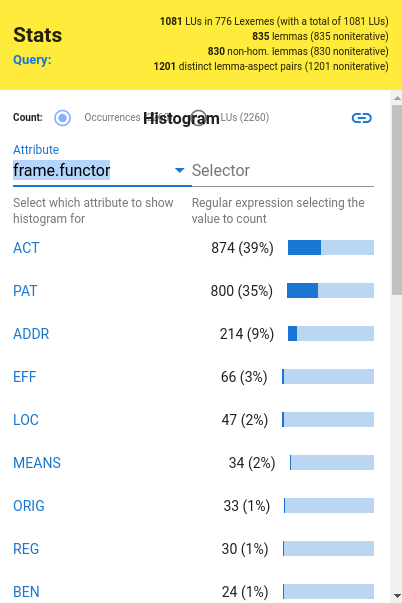
\includegraphics[width=\hsize]{images/histogram.png}
    \caption{\label{fig:histogram}The web-based UI showing a histogram of the frame functors}
\end{figure}

%------------------------------------------------
\subsection{Scripts}
The script module (\py{vallex.scripts}) provides a framework for running simple procedures over the
valency lexicon data. The scripts are loaded by the framework from a configurable directory. Each
file in this directory is a Python source file containing the definitions of the procedures.
The system currently recognizes five kinds of procedures: \emph{test}, \emph{transform}, \emph{compute} and \emph{map/reduce}.

\paragraph{Test} The test procedures are used to implement data validation for the lexicon. Each test
function receives a lexical unit as its argument.\footnote{Actually, there are four sub-types differing in what
argument is passed --- a collection of lexicons, a single lexicon, a single lexeme or a lexical unit;
for simplicity here and also in the paragraphs dedicated to other types of procedures we discuss only the sub-type receiving a lexical unit.}
It checks whether the unit satisfies the test and raises an appropriate exception if it doesn't. The framework
iterates over all lexical units passing them in turn to each test procedure and collecting the results. The
results are saved in the in-memory representation and can then be displayed to the user (\autoref{fig:test-result}).
\begin{figure}
    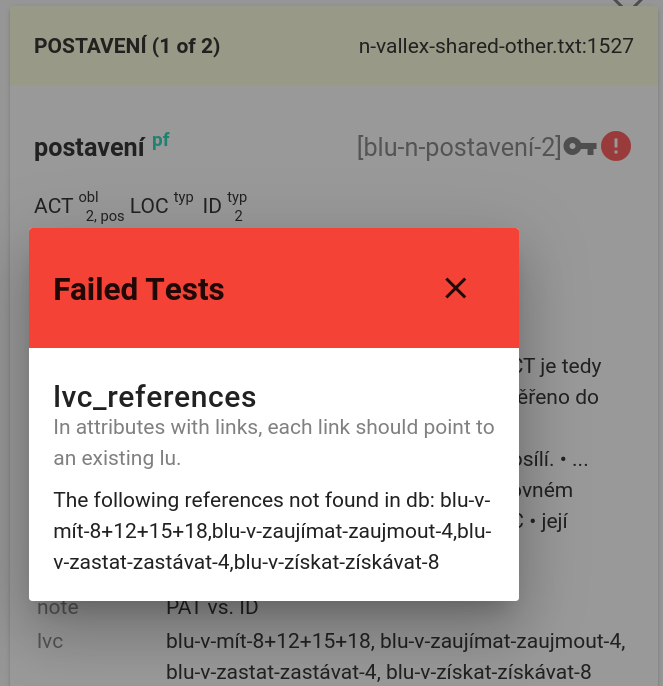
\includegraphics[width=\hsize]{images/test-result.png}
    \caption{\label{fig:test-result}The web-based UI showing the result of a data-validation run on a lexical unit.}
\end{figure}
The results are also annotated with the docstring of the test-procedure which can be used to provide human
readable explanation of the failed result. An example data validation test is provided in \autoref{fig:data-test-code}.
\begin{figure}
\small
%%\rrr{Figure 3 and Figure 4. Why not use the same test in both figures? That would provide more insight.}
% \begin{minted}{python}
% def test_lu_acc_without_deagent(lu):
%   """
%     Verbs that allow accusative form
%     of one of their complementations
%     must also allow the deagentive
%     diathesis.
%   """
%   forms = sum(
%      [fe.forms for fe in lu.frame.elements],
%      []
%   )
%   has_acc = '4' in forms or
%               'adj-4' in forms
% 
%   if not has_acc or lu.isReflexverb:
%     raise TestDoesNotApply
% 
%   deagent = 'diat' in lu.attribs and
%       'deagent' in lu.attribs['diat']._data
% 
%   if not deagent:
%       raise TestFailed()
% \end{minted}
\begin{minted}{python}
@requires('lumap')
def test_lu_lvc_references(lu, lumap):
  """
    In attributes with links, each link
    should point to an existing lu.
  """
  failures = []
  lvc_variants = [k for k in lu.attribs.keys()
                    if k.startswith('lvc')]
  if not lvc_variants:
    raise TestDoesNotApply
  applies = False
  for attrib in lvc_variants:
    if not \
      isinstance(lu.attribs[attrib]._data,
                 dict):
      continue
    refs = lu.attribs[attrib]._data['ids']
    if refs:
      applies = True
      for ref in refs:
        if not ref._id.startswith('@') \
           and ref._id not in lumap:
          failures.append(str(ref._id))
  if failures:
    raise TestFailed("The following \
             references not found in db: "
             +','.join(failures))
\end{minted}

\caption{\label{fig:data-test-code}An example of a data-validation procedure}
\end{figure}

\paragraph{Transform} The transform procedures can be used to implement one-time lexicon-wide changes, e.g.
renaming an attribute. They receive a lexical unit which they can modify and return.

\paragraph{Compute}\label{sec:computed} The compute procedures are similar to the transform procedures, but are used to implement dynamically computed properties which are \emph{not} saved back to the lexicon on disk.

\paragraph{Map/Reduce} The map/reduce procedures are used to perform more complicated analyses of the lexicon
for which a simple search/histogram does not suffice. Each map/reduce procedure consists of a pair of functions:
a \emph{mapper} and an (optional) \emph{reducer}. Each mapper receives a lexical unit as an argument and
uses a framework-provided \py{emit} function to emit a collection of \py{(key, value)} pairs. The framework
iterates over all lexical-units passing them to the mapper functions and collecting the resulting pairs. It then groups them by the \py{key} component and passes the groups to the reducer which can do further processing.
A default reducer which just counts the number of values for a given key is provided by the framework and is
used when no specialized reducer is provided by the user. Note that, although map/reduce is now commonly associated with
parallel processing, here all the mappers and reducers are run sequentially---the small size of the data does not justify
the additional complexity of parallel processing. We use map/reduce only as a familiar paradigm for structuring
analysis code.
\rrr{Could you potentially implement the map/reduce system in parallel form as well (even though that is not done currently)?}

%------------------------------------------------
\subsection{Output}\label{sec:output}

The output module provides tools to export lexicon data in various formats. In addition to built-in JSON
output (which is implemented in the data-layer), new formats can be defined using \emph{Jinja2} \cite{tool:Jinja2} templates.
Currently only a single txt format is provided which outputs the in-memory representation in the same
format that the annotators use. This can be used to check the fidelity of the in-memory representation
(by comparing it with the original source) and for normalizing the sources. In the future other formats
may be added, e.g., 
one of the XML-based internationally recognized formats such as XML:TEI or the RDF/XML serialization of the OntoLex-Lemon model.

%----------------------------------------------------------------------------------------
%	THE UI LAYER
%----------------------------------------------------------------------------------------

\section{The UI Layer}

Although the PyVallex system provides a command line UI for performing searches, computing histograms
and running batch scripts, it is expected that most of its users will prefer a nicer graphical user interface.
We have decided to provide the GUI as a web-based interface. This has several advantages. First, it allows
the system to be installed on a server and be accessible to users without forcing them to acquire the needed datasets
or requiring them to maintain the installation. Moreover, web-based technologies are very
common and basing the UI on them considerably lowers the barrier for new contributors/maintainers. It
is expected that even a person without a detailed knowledge of the system would be able to contribute simple modifications to the UI in a short amount of time. Finally, using a webview widget provided by the
\emph{Qt library} \cite{tool:Qt},
we can implement a simple local client based on the same code-base.

\subsection{Implementation}
The server-backend is a simple Python \emph{WSGI} \cite{tool:WSGI} application written in the \emph{Bottle.py} \cite{tool:bottle.py}
microframework. It uses an \emph{SQLite} database \cite{tool:SQLite} to store a JSON representation of the in-memory
data\footnote{The database is used solely as a method to allow safe concurrent access to the data.} and exposes a REST-based api which is consumed by the front end. The front end is a Javascript application written using the
\emph{Vue} framework \cite{tool:vue}  together with the
\emph{Vuetify} component library \cite{tool:Vuetify} to provide a familiar
\emph{Polymer}-style interface \cite{tool:polymer}.

\subsection{User Features}
\subsubsection{Searching}
By default, all lexemes in the lexicon are displayed in alphabetical order.
However, the GUI provides an interface for formulating queries (Section \ref{sec:query});
to improve user experience, all existing selectors are listed in a drop-down list (Figure \ref{fig:ui-search}).
To clarify the meaning of selectors, a help string may be provided;
the user may also click on the key icon next to any lexical unit
and see a full listing of the selector--value pairs for the given unit.



\begin{figure}
    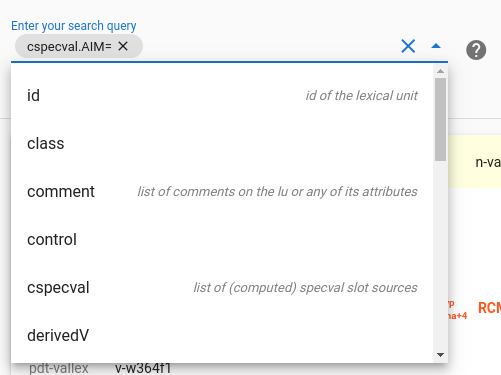
\includegraphics[width=\hsize]{images/ui-search.png}
    \caption{\label{fig:ui-search}The search field}
\end{figure}

\subsubsection{View modes}
Currently, two view modes are provided for lexical units:
in the Source View mode, the complete portion of the source file that corresponds to the given lexical unit is run through a simple regex-based syntax highlighter that mimics the function of the text editor known to the annotators.
On the other hand, the Default View mode is based on a template that can access the complete output of the parser (Section \ref{parser})
as well as computed properties not present in the source files (Section \ref{sec:computed})
and the full formatting capabilities of the \emph{Vue.js} framework.
A particularly useful feature of the Default View is the fact that linked lexical units
(such as source verbs of deverbal nouns or translation equivalents in case of our Russian and Polish lexicons)
can be displayed in a pop-up with a single click.
The two views can be compared in Figures \ref{fig:ui-lexical-unit-src} and \ref{fig:ui-lexical-unit}.

\begin{figure}
    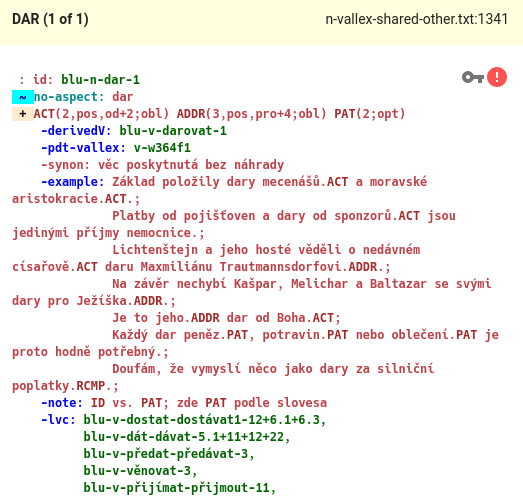
\includegraphics[width=\hsize]{images/ui-lexical-unit-src.png}
    \caption{\label{fig:ui-lexical-unit-src}The display of a lexical unit (Source View)}
\end{figure}

\begin{figure}
    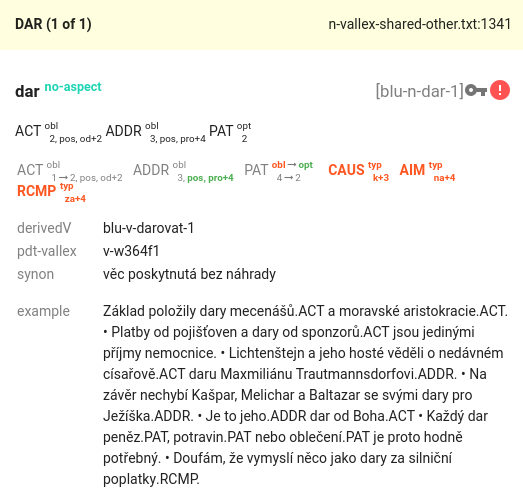
\includegraphics[width=\hsize]{images/ui-lexical-unit.png}
    \caption{\label{fig:ui-lexical-unit}The display of a lexical unit (Default View)}
\end{figure}


The \texttt{filter} method (Section \ref{sec:execute_query}) may be triggered from the settings menu as a selection of attributes to be displayed.
A simple interface for showing various histograms is also available (ibid.).


\subsubsection{Basic Editing}
Because of the assumption that the web-based GUI will not replace the existing annotation pipeline
(text files stored in a Subversion repository),
the current implementation does not provide editing functionality in the web-based interface.
Nonetheless, a simple component for editing a single (pre-existing) lexical unit is available
in the local client-side \emph{Qt}-based GUI,
so that annotators may quickly correct minor issues encountered while searching the data;
the client initially reads data from the working copy of the Subversion repository and stores a JSON
representation of this data in an \emph{SQLite} database for safe concurrent access.
The user can open an editor view (see \autoref{fig:ui-editing}) and do some edits. When the editor
view is closed, the system first checks that the state of the entry in the database has not changed since opening the editor, then parses the new textual form of the lexical unit and replaces the whole unit in the database,
also updating its in-memory representation. In case the unit has changed since the editing window was opened,
the user is warned and no changes are stored. Upon request, the contents of the \emph{SQLite} database can be output in the textual form back to the subversion repository the data was originally read from (making sure that any files changed in the meantime are backed up; see Section \ref{sec:output}); it is the users' responsibility to commit the changes, resolve conflicts etc.


\begin{figure}
    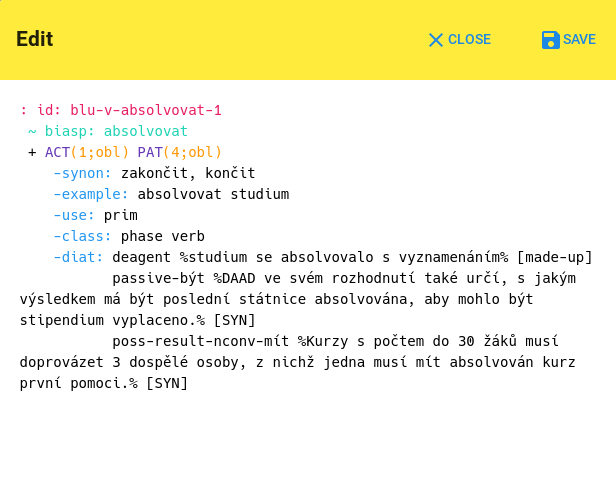
\includegraphics[width=\hsize]{images/ui-editing.png}
    \caption{\label{fig:ui-editing}A simple editor}
\end{figure}



%----------------------------------------------------------------------------------------
%	FUTURE WORK
%----------------------------------------------------------------------------------------
\section{Future work}
Some features of our old pipeline,
e.g.\ XML and PDF output,
have yet to be implemented in PyVallex.
PyVallex is currently only available in source code form\footnote{\url{https://gitlab.com/Verner/pyvallex}}, 
although we plan to publish it as pre-built
package in the PyPi package repository. The client-side \emph{Qt}-based GUI is now distributed as a stand-alone
executable file\av{s for Unix and Windows operating systems}.
\rrr{In what format is this? Is this operating system independent? (How accessible/usable is this to users on different operating systems?)}
Although this has some advantages (simplicity, easy updates), it has a significant
performance cost---the single file is basically a self-extracting archive which must unpack itself
every time the program is run.

While the client-side \emph{Qt}-based GUI allows for basic editing, it would be nice to incorporate this into
the web-based UI. This will require some form of user authentication/authorization to be implemented.
Eventually, the editing capabilities could be extended to allow for more comprehensive
edits (including creating new lexemes/lexical units). This would allow some annotators
to use the PyVallex system as the main or only tool to create or edit
lexicons, and external users to efficiently submit feedback on individual lexical units as well as suggest extensions of the lexicon.

Finally, the modular architecture of PyVallex which allows programmatic access to the data in a structured
way makes it an ideal tool for script-based examination of multiple revisions of the same data.
We therefore plan to implement additional tests for guarding the internal and mutual consistency of the annotation present in all four sister-projects that use the Vallex format: Vallex, NomVallex, RU-Vallex and PL-Vallex.

\subsection{Extending PyVallex for other projects}
A recent survey of lexicographic practices in Europe  has found that most projects use an in-house DWS rather than an off-the-shelf solution
\cite{KallasEtAl19lexicographic}.
Even though PyVallex is not primarily a DWS, it can be viewed as just another addition towards this trend.
One of the arguments for an in-house solution was the fact that the lexicographers on our teams are happy with the current setup:
the main source of truth about the lexicon data are files in the text-based Vallex format,
shared between annotators in a Subversion repository.
In contrast to XML-based formats such as XML:TEI \cite{XMLTEI2020}
and the RDF/XML serialization of the OntoLex-Lemon model \cite{BosqueGilGracia19OntoLex},
our format is compact and practical for direct and daily use by humans;
moreover, it is easy to inspect changes in the data with general-purpose diff tools.
This means that in order to build upon pre-existing software for the presentation, querying and editing of our lexicographic data,
we would have to write custom conversion scripts to and from the native format of those tools,
and create a pipeline allowing for continuous integration of changes coming from the Subversion.
However, once we have a parser for our format,
it is natural to use the resulting internal representation of the data as the input for queries, scripts, and output functions.
In short, the PyVallex framework is a result of the wish to enable developers to write a parser and then reuse the resulting representation for multiple purposes.
Although most of the current development of PyVallex concentrates on the Vallex-specific functions,
the general framework is ready to work with other data models as well.
We thank the anonymous referees for pointing out that as a first step towards adoption of PyVallex by other projects,
we could implement parsers and output functions for internationally recognized lexicon exchange formats.
In fact, we could go even further and make sure that the internal representation of lexicon data in PyVallex reflects the OntoLex-Lemon model.


\section{Acknowledgements}
The research reported in this paper has been supported by the projects No.\ 18-03984S (\textit{Between Reciprocity and Reflexivity: The Case of Czech Reciprocal Constructions}) and No.\ 19-16633S (\textit{Valency of Non-verbal Predicates}) of the  Czech Science Foundation (GA{\v{C}R}) and partially also by the \textit{LINDAT/CLARIN} project of the Ministry of Education, Youth and Sports of the Czech Republic (project No. LM2015071).

The first author was also supported by Charles University Research Centre program No.\ UNCE/SCI/022 and by the Progres grant Q14. Krize racionality a {modern\'\i} my\v{s}len\'\i.

This work has been using language resources stored and distributed by the \textit{LINDAT-CLARIN} project of the Ministry of Education, Youth and Sports of the Czech Republic, project No. LM2015071.

\av{We thank the anonymous referees for their valuable suggestions, and in particular the second referee for detailed comments about individual spots in the text.}

%----------------------------------------------------------------------------------------
%	BIBLIOGRAPHY
%----------------------------------------------------------------------------------------

%\printbibliography[title={Bibliography}] % Print the bibliography, section title in curly brackets

\section{Bibliographical References}
\label{main:ref}

\bibliographystyle{lrec}
\bibliography{example}

%----------------------------------------------------------------------------------------

\end{document}
